\documentclass[11pt]{article}
\usepackage[margin=0.75in]{geometry}
\usepackage{amsmath}
\usepackage{amssymb}
\usepackage{setspace}
\usepackage{graphicx}

\usepackage{color}
\definecolor{deepblue}{rgb}{0,0,0.5}
\definecolor{deepred}{rgb}{0.6,0,0}
\definecolor{deepgreen}{rgb}{0,0.5,0}
\usepackage{listings}

\DeclareFixedFont{\ttb}{T1}{txtt}{bx}{n}{12} % for bold
\DeclareFixedFont{\ttm}{T1}{txtt}{m}{n}{12}  % for normal

% Python style for highlighting
\newcommand\pythonstyle{\lstset{
    language=Python,
    basicstyle=\ttm,
    otherkeywords={self},             % Add keywords here
    keywordstyle=\ttb\color{deepblue},
    emphstyle=\ttb\color{deepred},    % Custom highlighting style
    stringstyle=\color{deepgreen},
    frame=tb,                         % Any extra options here
    showstringspaces=false            % 
}}


% Python environment
\lstnewenvironment{python}[1][]
{
    \pythonstyle
    \lstset{#1}
}
{}

    

\begin{document}

\title{ECE 4750 Lab 1: Iterative Integer Multiplier}
\author{Akshay Dongaonkar (akd54) \& Avinash Navada (abn44) \& Vivek Gaddam (vrg22)}
\maketitle

\section{Introduction}

In many programming algorithms, multiplication is a key step in driving the algorithm towards completion. 
Many digital signal processing algorithms spend most of their time multiplying values. 
Given our media heavy, highly connected Internet of Things (IoT), more signals will need to be processed.
Therefore, we have synthesized an iterative multiplier that supports the mul instruction as defined in the PARCv1 Instruction Set Architecture (ISA).
Eventually, this multiplier will be a module in a fully synthesizable multicore processor.

We implemented two multiply designs: the first is a fixed latency, 34 cycle iterative multiplier while the second is a variable latency
iterative multiplier with bounds of 3 to 34 cycles.
While we do not expect much additional overhead on clock frequency in our variable multiplier,
we expect a significant increase in area and energy.
Given the technology constraints we face today, (focus on energy, large die sizes, etc),
we expect our variable multiplier to be superior in most implementations. 


\section{Project Management}

\section{Baseline Design}

The baseline design works on the following interface: 
given a 64 bit message containing our operands, a clock signal,
and required signals to conform to the val/rdy microprotocol,
output the lower 32 bits of the multiplication to your consumer.
This interface is shown in Figure $1$.
Our algorithm for computing the multiplication is as follows.
If the least significant bit (lsb) of the second operand (call it $b$) is 1, add it to an accumulator.
Then, shift your first operand (call it $a$) left by one bit and the second operand to the right logically by one bit.
This is the first algorithm we are taught when we learn to multiply.
The pseudocode for this is shown in Figure 2. 

Our implementation follows the structure of this pseudo-code very closely.
We have three registers, one each for $a$, $b$, and $result$ (our accumulator).
We have 2 shifters, one logical left shifter and one logical right shifter. 
We have an equivalent multiplexor for the clause that adds to our accumulator if the lsb of $b$ is $1$.

However, the control logic and the data flow are not implemented as a monolithic design.
Instead, we implement a \textit{control-datapath split.}
The control module sends control signals to the datapath module, altering the flow of data into the registers.

  

\section{Alternative Design}

\section{Testing Strategy}

\section{Evaluations and Conclusion}

\begin{figure}
\centering
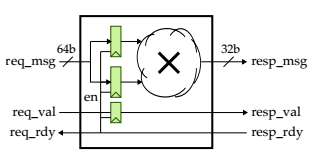
\includegraphics[scale=0.5]{FLmodel}
\caption{Interface for our model. Notice that req/resp,val/rdy signals are part of the val/rdy microprotocol}
\end{figure}

\begin{figure}
\centering
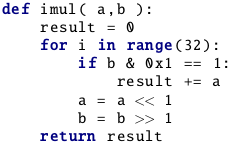
\includegraphics[scale=0.9]{imul}
\caption{Pseudocode for our baseline multiply algorithm}
\end{figure}

\begin{figure}
\centering
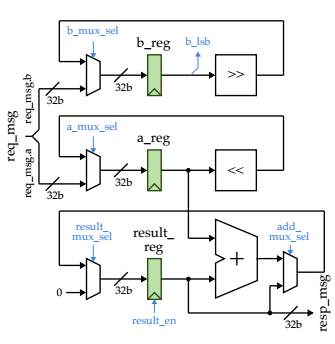
\includegraphics[scale=0.6]{Datapath}
\caption{Datapath Diagram. Again, the structure mimics the pseudocode.}
\end{figure}


\end{document}
